%% It is just an empty TeX file.
%% Write your code here.
\subsection{Casos simulados - II Enfermería}
Los siguientes casos descritos fueron pensados en su totalidad por María Fuencisla Sanz para el curso 2022/2023, en el contexto de las simulaciones y seminarios para la asignatura de Prácticas Clínicas (II Grado en Enfermería). El concepto general que subyace a todos ellos es, por una parte, evaluar las competencias técnicas (correcta toma de signos vitales (dolor, tensión arterial, saturación, frecuencias respiratoria y cardiaca, temperatura y glucemia (si el caso indicaba diabetes)), correcta higiene del paciente encamado, correcta administración de medicamentos), y por otro, desarrollar una serie de habilidades como el pensamiento crítico, comunicación interpersonal y evaluación de la gestión al estrés y consejos en el plano de la comunicación con el entorno del paciente.

Se diferencian dos tipos de casos, ambos se evaluarán con la rúbrica contenida en la tabla \ref{tab:PlanXVII:RubricaUCM}: el caso de higiene/Simulación del paciente encamado, que es una higiene normal, hecha por dos alumnas y que como único elemento a tener en cuenta es si el paciente es o no continente, decisión que se tomará en el momento. Los casos de simulación propiamente dichos (ver esquema en la figura \ref{fig:PlanXVII:FlujogramaGeneral}), desarrollados individualmente, tienen un componente de <<gestión de eventos emergentes/urgentes>>, esto es, hay un suceso interruptor en el que el alumnado tendrá que decidir si lo soluciona, bien movilizando al paciente por dolor, bien dándole algún tipo de medicamento o remedio o bien avisando en caso de que no pueda gestionarlo por si mismos. 

\begin{figure}[H]
    \centering
	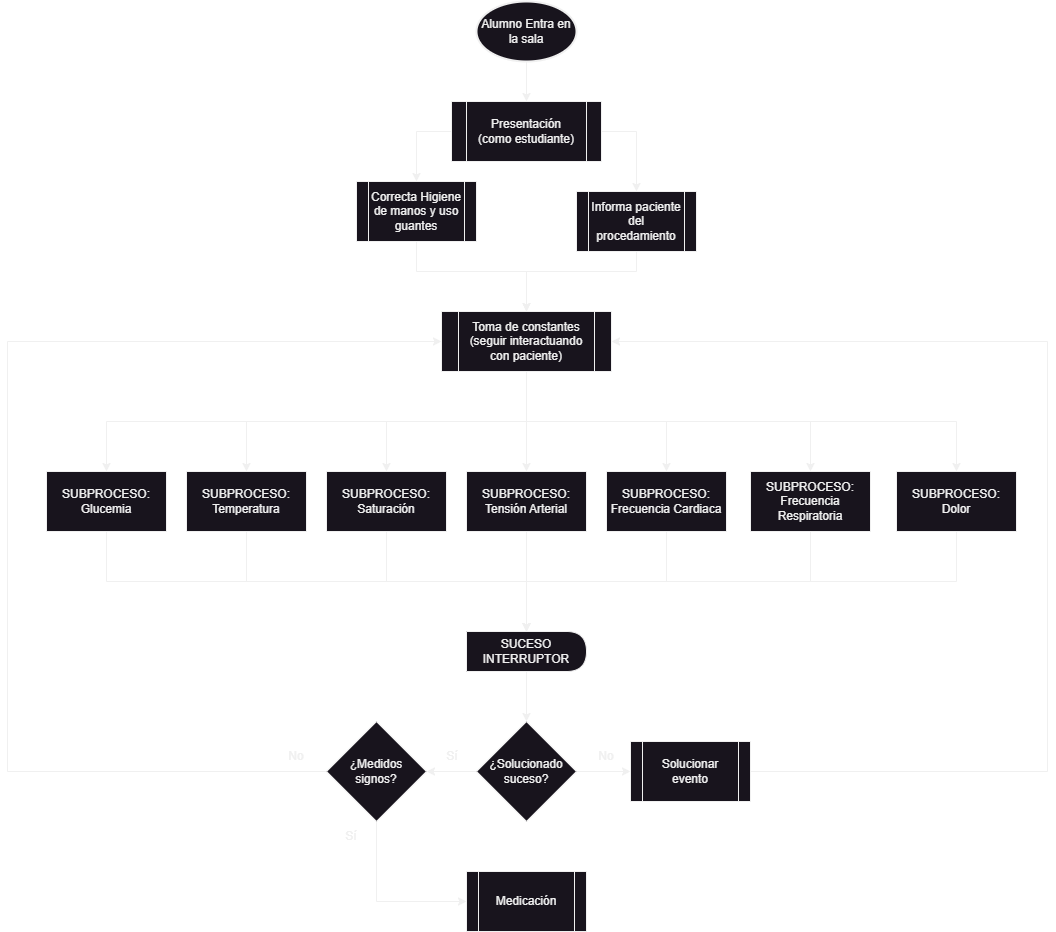
\includegraphics[width=0.8\textwidth]{./imagenes/ACV-AdSC-CasosIIEnfermeria-ResolucionGeneral.png}
	\caption{\label{fig:PlanXVII:FlujogramaGeneral}Flujograma general de los casos.}
\end{figure}


